\chapter{Preliminaries}
\label{chapter:mathematical-preliminaries}

The ultimate interest of this dissertation is to introduce a style of non-monotonic reasoning, originally situated
in propositional logic, into Formal Concept Analysis. We use the first chapter to recall some of the more
foundational ideas relating to topics which will be developed further on. In addition, we use this chapter as an
opportunity to clarify the notation which will be deployed throughout the remainder of this work.

This chapter begins by discussing notions in \textit{order} and \textit{lattice theory}, then moving onto
\textit{closures} and \textit{Galois connections}, and concluding with a brief introduction to
\textit{propositional logic} and some more general notions relating to logic.

\section{Order and Lattice Theory}
\label{section:order-theory}

In substantially different ways, the two areas on which this work is based---non-monotonic reasoning via
preferential semantics, and Formal Concept Analysis---both depend on notions from the theory of mathematical
orders. We recount some of the necessary, and unnecessary but interesting, ideas in the following subsections. The
proceeding follow largely from the treatments by \cite{davey2002introduction} and \cite{bergman2015invitation}.

\subsection{Orders}
\label{subsection:orders}

A \textit{binary relation} \index{binary relation} $R$ over the sets $X$ and $Y$ is a set of ordered pairs
$\op{x,y}$ where $x \in X$ and $y \in Y$. It is always the case that $R \subseteq X \times Y$, and so in the case
where at least one of the sets is infinite, the $R$ may also be infinite. We may choose to express that
$\op{x,y}\in R$ using infix notation and write $xRy$, which tells us that $R$ relates $x$ to $y$. As expected,
$(x,y) \not \in R$ means that $x$ is not related to $y$ by $R$; of course, this may be true while $(y,x) \in R$.

Certain binary relations, satisfying specific properties, occur frequently enough to warrant their own
denomination. One such relation, is called a \textit{partial order}.

\begin{definition}
	\label{definition:partial-order} \index{partial order}

	A \textit{partial order} is a binary relation $\preceq \; \subseteq X \times X$ that satisfies the properties:
	\begin{align}
		\text{(Reflexivity)}\quad  & x \preceq x                                      \\
		\text{(Antisymmetry)}\quad & x \preceq y \tand y \preceq x \timpl x = y       \\
		\text{(Transitivity)}\quad & x \preceq y \tand y \preceq z \timpl x \preceq z
	\end{align}
	for all $x,y,z \in X$.
\end{definition}

Frequently, ``preference'' is used as a metonym for an ordering. In this context, writing \say{element $x$ is
	preferred to $y$} should be interpreted to mean that $(x, y) \in \; \preceq$, or simply $x \preceq y$. The
metaphorical use of ``preference'' will become more relevant in \Cref{chapter:defeasible-reasoning}.

To indicate that $x \preceq y$ but $x\not = y$, we may write $x \prec y$. In the event where $x \not \preceq y$
and $y \not \preceq x$---i.e., that $x$ and $y$ are incomparable---we may write $x \parallel y$. From a partial
order it is quite natural to describe the notion of a \emph{strict partial order}.

\begin{definition}
	\label{definition:strict-partial-order} \index{partial order! strict}

	A \textit{strict partial-order} is a binary relation $\prec \; \subseteq X \times X$ that satisfies:
	\begin{align}
		\text{(Irreflexivity)}\quad & x \nprec x                                 \\
		\text{(Asymmetry)}\quad     & x \prec y \timpls y \nprec x               \\
		\text{(Transitivity)}\quad  & x \prec y \tand y \prec z \timpl x \prec z
	\end{align}
	for all $x,y,z \in X$.
\end{definition}

An \textit{ordered set} is a pair $(X, \preceq)$. $X$ may be called the \textit{carrier set} for which $\preceq \;
	\subseteq X \times X$ is the \textit{underlying order}. For a subset $Y \subseteq X$, $Y$ may inherit the order
associated with $X$ but restricted to $Y$; unless otherwise stated it is assumed that subsets of carrier sets
inherit the underlying order. Ordered sets may be described visually by \textit{Hasse diagrams}
\cite{Huth_Ryan_2004}. \index{Hasse diagrams} \index{ordered set}

\begin{figure}[H]
	\centering
	\small
	\begin{subfigure}{0.3\textwidth}
		\centering
		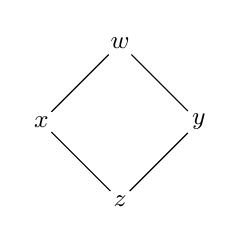
\begin{tikzpicture}[
				every node/.style={ circle,
						% fill=black,
						text=black, inner sep=1.2pt, font=\small } ] \node (w) at (0,1) {$w$}; \node (y) at (-1,0) {$x$}; \node (z) at
			(1,0) {$y$}; \node (x) at (0,-1) {$z$};

			\draw (w) -- (y);
			\draw (w) -- (z);
			\draw (y) -- (x);
			\draw (z) -- (x);
		\end{tikzpicture}
		\subcaption{$(A,\preceq_A)$} \label{subfigure:partial-order-a}
	\end{subfigure}
	\begin{subfigure}{0.3\textwidth}
		\centering
		\begin{tikzpicture}[
				every node/.style={ circle,
						% fill=black,
						text=black, inner sep=1.2pt, font=\small } ] \node (y) at (-1,0) {$\phi$}; \node (z) at (1,0) {$\psi$}; \node (x)
			at (0,1) {$\omega$};

			\draw (y) -- (x);
			\draw (z) -- (x);
		\end{tikzpicture}
		\subcaption{$(B,\preceq_B)$} \label{subfigure:partial-order-b}
	\end{subfigure}
	\caption{The Hasse diagrams of two partially ordered sets} \label{figure:hasse-diagram}
\end{figure}

As an illustrative example, from the ordered set in \Cref{subfigure:partial-order-a} it can be read that $z
	\preceq x$, as there is a (strictly) upward path from $z$ to $x$. In fact, it is clear that $z \preceq w, x,y,z$,
or that \say{$z$ is preferred to every other element in $A$}. Such an element is said to be \textit{minimal}.

More formally, an element $x \in X$ is \textit{minimal} with respect to an ordering $\preceq$ on its carrier set
if there is no distinct element $y \in X$ where $y \preceq x$. Conversely, $y$ is the maximal element if there is
no distinct $x \in X$ where $y \preceq x$. There may of course be multiple minimal or maximal elements, for
example $\phi$ and $\psi$ in \Cref{subfigure:partial-order-b}. For finite orders, there is always at least one
minimal and maximal element. This condition is not true for all infinite orderings; consider for example the set
of integers. In the case where $x$ is the unique minimal element it is called the \textit{minimum}. This may be
phrased equivalently as $x \preceq y$ for all $y \in X$. The dual notion of the \textit{maximum} is defined in the
expected way.

\index{maximum} \index{minimum} \index{maximal} \index{minimal}

Frequently ordered sets are mapped onto other ordered sets. Suppose that $\varphi \colon X \to Y$ is a mapping
from $(X,\preceq_X)$ to $(Y,\preceq_Y)$. Then, $\varphi$ is called an \textit{order-preserving}, or
\textit{isotone}, map when $x \preceq_X$ implies $\varphi(x) \preceq_Y \varphi(y)$. If $\varphi$ is injective and
$x\preceq_X y$ if and only if $\varphi(x) \preceq \varphi(y)$ then it is called an \textit{order-embedding}. Note
that an order-embedding is necessarily order-preserving. Finally, $\varphi$ is an \textit{order-isomorphism}, or
just an \textit{isomorphism}, if it is an order-embedding that is also surjective. The dual notion to an
order-preserving map is an \textit{order-reversing} (or, \textit{antitone}) map. We say that two orders are
\textit{dually isomorphic}, or \textit{order-anti-isomorphic}, if there is an order-reversing bijection between
them.

\subsection{Lattice Theory}
\label{subsection:lattice-theory}

Lattice theory studies partially ordered sets that behave well with respect to certain properties involving upper
and lower bounds \cite{davey2002introduction}. Later on it will be shown that these properties make them
particularly well-suited to modelling hierarchical structures. Given an ordered set $(X,\preceq)$ and a subset $Y
	\subseteq X$ which inherits the order, the set of upper bounds of $Y$ is defined as
\[
	{Y}^{u}\coloneqq \{x \in {X}\mid \forall y \in {Y}: y \preceq x\}.
\]
The set of lower bounds, ${Y}^{l}$, is defined dually. If ${Y}^{u}$ has a minimum element $y$, then $y$ is the \textit{supremum} of $Y$. Dually, if $Y^l$ has a maximum element $x$, then $x$ is the infimum of $Y$. The supremum and infinum may also be referred to as the \textit{least upper bound} and \textit{greatest lower bound}, respectively.

\index{upper bound} \index{lower bound} \index{lattice!join} \index{lattice!meet}

Instead of talking about the supremum of two elements $x,y \in {X}$, we opt for the term \textit{join} and write
$x \vee y$, or $\bigvee {Y}$. Instead of infimum, we say \textit{meet} and write $x \wedge y$, or $\textstyle
	\bigwedge {Y}$. With these definitions of meets and joins in mind, we are able to define a lattice as:

\begin{definition}
	\label{definition:lattice}

	Given a partially ordered set $({L}, \preceq)$ is a \textit{lattice} if for every pair $x, y \in {L}$ the join $x
		\vee y$ and meet $x \wedge y$ exist, and are unique. ${L}$ is a \textit{complete lattice} if for every subset
	${M}\subseteq {L}$ both $\bigvee {M}$ and $\bigwedge {M}$ exist in ${L}$.
\end{definition}

\index{lattice!bounded}

A lattice $({L},\preceq)$ is \textit{bounded} if there exists an element $x \in {L}$ such that $x \vee y = x$ for
all $y \in {L}$, and there exists an element $z \in {L}$ with $z \wedge y = z$ for all $y \in {L}$. In other
words, a bounded lattice has a maximum and minimum element. Frequently these these elements are referred to as
\textit{top} and \textit{bottom} elements, respectively. It is not difficult to spot that every complete lattice
is bounded---in fact this is true by definition of a complete lattice---as a corollary every finite lattice is
also bounded.

% \begin{remark} The lattice $(\mathbb{Z}, <)$, constructed by imposing the natural order over the integers, is an example of an
% lattice that is not bounded. \end{remark}

\begin{example}
	\label{example:lattice of naturals}

	The set of natural numbers $\mathbb{N}$ forms a complete lattice when ordered by divisibility, sometimes called
	the \textit{division lattice}.
	\begin{figure}[H]
		\centering
		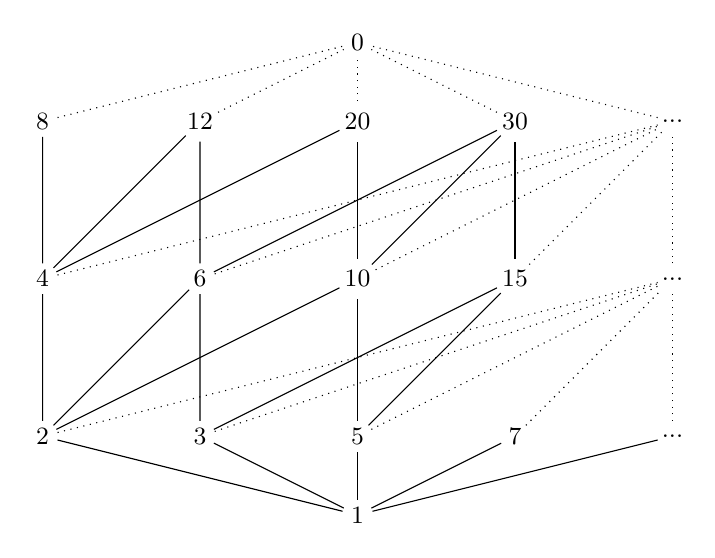
\begin{tikzpicture}[
				every node/.style={ circle,
						% %fill=black,
						text=black, inner sep=1.2pt, font=\small } ]

			\node (root) at (0,0) {$1$};
			\node (2) at (-4,1) {$2$};
			\node (3) at (-2,1) {$3$};
			\node (5) at (0,1) {$5$};
			\node (7) at (2,1) {$7$};
			\node (C) at (4,1) {$...$};
			\node (4) at (-4,3) {$4$};
			\node (6) at (-2,3)
			{$6$};
			\node (10) at (0,3) {$10$};
			\node (15) at (2,3) {$15$};
			\node (C1) at (4,3) {$...$};
			\node (8) at (-4,5) {$8$};
			\node (12) at (-2,5) {$12$};
			\node (20) at (0,5) {$20$};
			\node (30) at (2,5) {$30$};
			\node (C2) at (4,5) {$...$};
			\node (top) at (0,6){$0$};

			\draw (root) -- (2) -- (4) -- (8);
			\draw (4) -- (12);
			\draw[dotted] (12) -- (top);
			\draw (4) -- (20);
			\draw[dotted] (4) -- (C2);
			\draw[dotted] (8) -- (top);
			\draw (2) -- (6);
			\draw (6) -- (30);
			\draw[dotted] (6) -- (C2);

			\draw (2) -- (10);
			\draw (10) -- (20);
			\draw (10) -- (30);
			\draw[dotted] (10) -- (C2);
			\draw[dotted] (2) -- (C1);

			\draw (root) -- (3) -- (6) -- (12);
			\draw (3) -- (15);
			\draw (15) -- (30);
			\draw[dotted] (15) -- (C2);
			\draw[dotted] (C1) -- (C2);

			\draw[dotted] (3) -- (C1);

			\draw (root) -- (5) -- (10);
			\draw (5) -- (15);

			\draw[dotted] (5) -- (C1);
			\draw[dotted] (7) -- (C1);
			\draw[dotted] (C) -- (C1);
			\draw[dotted] (20) -- (top);
			\draw[dotted] (30) -- (top);
			\draw[dotted] (C2) -- (top);
			\draw (root) -- (7);
			\draw (root) -- (C);
		\end{tikzpicture}
		\caption{The Division Lattice $(\mathbb{N}, \leq)$} \label{figure:complete-lattice}
	\end{figure}

	In the division lattice, the join operation corresponds to the \textit{least common multiple}, and the meet
	operation to the greatest common divisor. The bottom element of this lattice is $1$ as it divides every other
	natural number, while the top element is $0$ since it is divisible by all other naturals and is not a divisor of
	any. Although the division lattice is infinite, it is a complete lattice.
\end{example}

\subsubsection{Lattices as algebraic structures}
\label{subsubsection:lattices-as-algebraic-structures}

Lattices may also be considered from an algebraic perspective. Although, as we will soon show, the algebraic and
order-theoretic perspectives coincide, it is frequently beneficial for one's intuition to be able to switch
between these two perspectives.

Consider a set $L$ equipped with a binary operation $\vee$ that satisfies the following properties
\begin{align}
	\text{(Idempotence)}   & \quad x \vee x = x \label{eq:idempotence}                            \\
	\text{(Commutativity)} & \quad x \vee y = y \vee x \label{eq:commutativity}                   \\
	\text{(Associativity)} & \quad (x \vee y) \vee z = x \vee (y \vee z) \label{eq:associativity}
\end{align}
for all elements $x,y,z \in L$.

From the algebraic structure $(L, \vee)$ one can induce a \textit{unique} partial order $\preceq$ on $L$ by
construction of the relation $\{( x, x \vee y) \mid x,y \in L \}$ \cite{bergman2015invitation}. The structure $(L,
	\vee)$ is called an algebraic \textit{join semilattice}, and $\preceq$ its \textit{underlying partial order}. The
relation can equivalently be described as \say{$x \preceq y$ if and only if $x \vee y = y$}.

\begin{example}
	\label{example:power-set-lattice}

	Consider the set $S = \{1,2,3\}$ and the union operation $\cup$. From $(\pset{S}, \cup)$ we can induce the order
	relation characterised by the set $\{(X, X \cup Y) \mid X,Y \subseteq S \}$. Frequently, this kind of ordering is
	called the \textit{set inclusion order}.
	\begin{figure}[H]
		\centering
		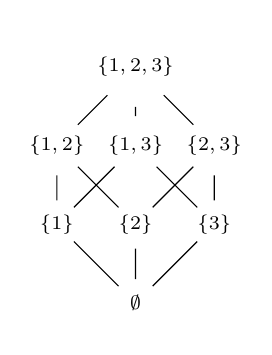
\begin{tikzpicture}[every node/.style={ circle,text=black, inner sep=0pt, minimum size=6mm, font=\scriptsize } ]
			\node (root) at (0,0) {$\emptyset$};
			\node (1) at (-1,1) {$\{1\}$};
			\node (2) at (0,1) {$\{2\}$};
			\node (3) at (1,1) {$\{3\}$};% no extra padding% ← choose one diameter for all nodes%

			\node (12) at (-1,2) {$\{1,2\}$};
			\node (13) at (0,2) {$\{1,3\}$};
			\node (23) at (1,2) {$\{2,3\}$};
			\node (123) at (0,3) {$\{1,2,3\}$};

			\draw (root) -- (1) -- (12) -- (123);
			\draw (root) -- (2) -- (12);
			\draw (root) -- (3) -- (23) -- (123);
			\draw (1) -- (13) -- (123);
			\draw (2) -- (23);
			\draw (3) -- (13);
		\end{tikzpicture}
		\caption{The underlying order of $(\pset{S}, \cup)$} \label{figure:set-inclusion-order}
	\end{figure}
	%
	From the Hasse diagram in \Cref{figure:set-inclusion-order} representing this order, we observe that the $\cup$
	binary relation corresponds to the $\vee$ described in \Cref{definition:lattice}.
\end{example}
\index{lattice!semilattice}

Instead, considering the structure $(L, \wedge)$ where $\wedge$ is a different binary operation on $L$ satisfying
the same properties \Crefrange{eq:idempotence}{eq:associativity}, a partial order may be constructed by
considering the set $\{( x,y) \mid x \wedge y = x \tand x,y \in L\}$. The structure $(L, \wedge)$ is called a
\textit{meet semilattice}.

It is an obvious next step to wonder how these two algebraic structures might be related. Fix a set non-empty set
$L$ with the two binary operations, $\vee$ and $\wedge$, introduced in the prior paragraphs. We have already seen
that the underlying order of the join semilattice can be described as $x \preceq y$ if and only if $x \vee y = y$,
while the underlying order of the meet semilattice is described by $x \preceq y$ if and only if $x \wedge y = x$.
These two partial orders are \textit{compatible} under the following condition:
\begin{align}
	\text{(Compatibility)} & \quad x \vee (x \wedge y) = x & \text{(resp.)} & \quad x \wedge (x \vee y) = x
\end{align}
Compatibility (which is sometimes also called \textit{absorption}) is satisfied when the underlying orders of both
semilattices refer to the same partial order. The property can be rewritten as $x \vee y = y$ if and only if $x
	\wedge y = x$. The formal definition of an algebraic lattice is given below:

\begin{definition}
	\label{definition:algebraic-lattice}

	The algebraic structure $(L, \vee, \wedge )$, where $L$ is a set and $\vee, \wedge$ are two binary operations on
	$L$, is a \emph{lattice} if both binary operations satisfy \textit{idempotence, commutativity,} and
	\textit{associativity} as well as \textit{absorption}.
\end{definition}

\textcolor{red}{NEED TO INCLUDE DEFN OF DISTRIBUTIVE LATTICES \& PARAGRAPH BEFORE LAST THEOREM}

\begin{lemma}
	\label{lemma:the-connecting-lemma}

	If $({L},\preceq)$ is a lattice with $x, y \in {L}$, then the following are equivalent:
	\begin{enumerate}
		\setlength{\itemsep}{0pt}
		\setlength{\parsep}{0pt}

		\item $x \preceq y$;

		\item $x \vee y = y$;

		\item $x \wedge y = x$.
	\end{enumerate}
\end{lemma}

Moving forward, the distinction between the algebraic and order-theoretic perspectives on lattices is not
maintained. Rather, we will tacitly adopt whichever viewpoint best suits the surrounding context. Lattices are
central to Formal Concept Analysis, and will be visited again in \Cref{chapter:formal-concept-analysis}.

\section{Closures \& Galois Connections}
\label{section:closure-systems}

\subsection{Closure Systems}

It is often useful to describe subcollections of elements within a larger set that are \emph{closed} under certain
structural properties. For example, in a partially ordered set $(X, \preceq)$, consider an element $x \in X$ and
the set of all elements $y \in X$ such that $x \preceq y$. If the order relation is given by $\{q \preceq x, x
	\preceq y,\, y \preceq z\}$, it is not sufficient to consider only the subset $\{y\}$, since partial orders are
reflexive and transitive. Conversely, the set $\{q,x,y,z\}$ is also not ideal, since it includes $q$ which does
not correspond to the sought property.

This operation corresponds to finding the \textit{upper set} of $x$. It is quite natural to think of the problem
of finding the closure under this operation as an iterative process of accumulating elements. That is, starting
with $\{x\}$, adding $\{y\}$, then $\{z\}$ until there are no more elements that may be added. Then, one has
reached a \textit{fixed-point}. This perspective is quite limiting, as it is unable to handle closed sets that
infinite. For example, finding all multiples of of $3$.

Instead, we consider the more abstract notion of a closure operator:
%
\begin{definition}
	\index{closure!operator} \label{definition:closure-operator}
	%
	A \emph{closure operator} on a set $S$ is a function $\varphi \colon \pset{S}\to \pset{S}$ assigning each subset
	of $S$ to its closure. A closure operator satisfies the following properties
	\begin{align}
		\text{(Monotony)}\quad    & X \subseteq Y \timpls \varphi(X) \subseteq \varphi(Y) \\
		\text{(Extensivity)}\quad & X \subseteq \varphi(X)                                \\
		\text{(Idempotency)}\quad & \varphi(X) = \varphi\big(\varphi(X)\big)
	\end{align}
	%
	for all $X,Y \subseteq S$.
\end{definition}
%
Formally, a set is \textit{closed} with respect to a closure operator if applying the operator does not add any
new elements. From the initial example, define $\upsilon$ as the closure operator mapping subsets of $X$ to to
their upper sets $\upsilon(X)$. Then, $\{x\} \mapsto \{x,y,z\}$. It may then be of further interest to study the
collection of upper sets of $X$. More generally, the study of closed sets relative to a given closure operator.
This is the study of \textit{closure systems}.

\begin{definition}
	\index{closure!system} \label{definition:closure-system}

	A \emph{closure system} on a set $S$ is a family of subsets $\mathcal{C}\subseteq \pset{S}$ containing the set $S$
	itself and the intersection of any subsets of $\mathcal{C}$, and so if $\mathcal{D}\subseteq \mathcal{C}$ then
	$\bigcap \mathcal{D}\in \mathcal{C}$.
\end{definition}

Aside from name, it is not immediately obvious how this definition of a closure system is related to the prior
motivation, which discussed studying collections of sets that are closed under a respective closure operator. The
following theorem confirms that they are indeed \textit{cryptomorphic} \cite{CASPARD2003241}.

\begin{theorem}
	\label{theorem:relation-closure-operator-systems}

	Let $\mathcal{C}$ be a closure system on $S$, then the function $\varphi : \pset{S} \to \pset{S}$ where
	\[ \varphi(Y) = \bigcap \, \{D \in \mathcal{C}\mid Y \subseteq D\} \]
	for $Y \subseteq S$, defines a closure operator on $S$. Conversely, if $\varphi \colon \pset{S} \to \pset{S}$ is a closure operator on $S$, then the collection of sets described by
	\[
		\{\, \varphi(X) \mid X \subseteq S \, \}
	\]
	defines a closure system on $S$.
\end{theorem}

For some intuition on the connection between closure operators and intersections, consider again the function
$\upsilon$, which maps subsets of $X$ to their up-sets. Let $A$ be the intersection $\upsilon(B) \cap \upsilon(C)$
of two up-sets, and suppose, for the sake of argument, that $A \neq \upsilon(A)$. In other words, while
$\upsilon(B)$ and $\upsilon(C)$ are closed, $A$ is not. Then there must exist an element $x \in \upsilon(A)$ with
$x \notin A$. By the definition of $\upsilon$, there is some $y \in A$ such that $y \preceq x$. Since $A \subseteq
	\upsilon(B)$ and $A \subseteq \upsilon(C)$, and also that these sets are bot closed, it must be that $x \in
	\upsilon(B)$ and $x \in \upsilon(C)$. But then $x \in A$. Hence our initial assumption must be false: the
intersection of two up-sets is itself an up-set, and therefore closed under $\upsilon$.

\begin{theorem}
	\label{theorem:closure-systems-lattices}

	Let $\varphi$ be a closure operator on the set $S$. Then the closure system given by $\{\,\varphi(X) \mid X
		\subseteq S\,\}$ forms a complete lattice under the inclusion order, where meets and joins are given by
	\[
		\underset{i \in I}\bigwedge X_{i}= \underset{i \in I}\bigcap X_{i},
	\]
	\[
		\underset{i \in I}\bigvee X_{i}= \varphi(\underset{i \in I}\bigcup X_{i}).
	\]
\end{theorem}

[NEED TO ADD A PARAGRAPH HERE]
%TODO lattice description for closure operator

\subsection{Galois Connections}
\label{subsection:galois-connections}

Galois connections describe a particular correspondence between two ordered sets \cite{bergman2015invitation}. We
will spend a bit of time describing Galois connections, as they are fundamental to FCA, and closely related to
ideas around closures.

\begin{definition}
	\label{definition:antitone-galois-connection}
	Let $(X,\preceq)$ and $(Y,\preceq)$ be two partially ordered sets. Then an \emph{antitone Galois connection} is a pair of antitone maps $\varphi \colon X \to Y$ and $\psi \colon Y \to X$ such that
	\[
		x \preceq \psi(y) \tiff y \preceq \varphi(x).
	\]
	for all $x \in X$ and $y \in Y$.
\end{definition}

Galois connections may not always refer to a pair of antitone maps. However, since we are only interested in those
that do, the ``antitone'' descriptor will be dropped in future. We recall several propositions about Galois
connections, which serve to provide further intuition \cite{ganter2024formal}.

\begin{proposition}
	\label{proposition:1}

	Let $(\varphi, \psi)$ refer to the same pair of maps constituting a Galois connection, then
	\begin{align}
		\quad & x \preceq_{X}x' \,\timpls \,\varphi (x') \preceq_{Y}\varphi (x) \label{equation:ord_galois-1}
		\\
		\quad & y \preceq_{Y}y' \, \timpls \,\psi (y') \preceq_{X}\psi (y) \label{equation:ord-galois-2}
		\\
		\quad & x \preceq_{X}\psi \big(\varphi (x)\big) \, \tand \, y \preceq_{Y}\varphi \big(\psi (y)\big)
		\label{equation:ord-galois-3}
	\end{align}
\end{proposition}

\Cref{equation:ord_galois-1,equation:ord-galois-2} are really just rephrasings of the definition of a Galois
connection. \Cref{equation:ord-galois-3} shows that the compositions $\varphi \circ \psi$ and $\psi \circ \varphi$
are extensive. \lucas{Maybe we should add a proof here?}

% \begin{proposition}
% 	\label{proposition:fundamental-galois}
%
% 	Let $(\varphi, \psi)$ refer to the same pair of maps constituting a Galois connection, then
% 	\begin{align}
% 		\quad & x \preceq_{X}\psi (y) \tiff y \preceq_{Y}\varphi (x) \label{equation:ord-galois-4}
% 	\end{align}
% 	for all $x \in {X}, y \in {Y}$.
% \end{proposition}

\begin{proposition}
	\label{proposition:monotonicity-of-galois}

	Let $(\varphi, \psi)$ refer to the same pair of maps constituting a Galois connection, then
	\begin{align}
		\quad & x \preceq_x x' \timpls \psi\big(\varphi(x)\big)  \preceq_X \psi \big(\varphi(x')\big), \tand \\
		\quad & y \preceq_y y' \timpls \varphi\big(\psi(y)\big) \preceq_Y \varphi\big(\psi(y')\big)
	\end{align}
	for all $x \in {X}, y \in {Y}$.
\end{proposition}

\begin{proposition}
	\label{proposition:galois-idem}

	Let ($\varphi, \psi$) refer to the same pair of maps constituting a Galois connection, then
	\begin{align}
		\varphi (x) = \varphi \Big( \psi \big( \varphi (x)\big) \Big) & \quad \text{and}\quad \psi (y) = \psi \Big( \varphi \big( \psi (y)\big) \Big)
	\end{align}
	for all $x \in {X}, y \in {Y}$.
\end{proposition}

By \Cref{proposition:1,proposition:monotonicity-of-galois,proposition:galois-idem} it follows that the two
compositions constructed from a Galois connection are monotone, extensive, and idempotent. In other words, they
are closure operators.

\begin{proposition}
	\label{proposition:galois-connections-closure-operators}

	Let ($\varphi, \psi$) refer to the same pair of maps constituting a Galois connection, then
	\[
		x \mapsto \psi \big(\varphi(x)\big) \quad \text{and}\quad y \mapsto \varphi \big(\psi (y)\big)
	\]

	are \textit{monotone, extensive} and \textit{idempotent} and thus constitute closure operators on ${X}$ and ${Y}$,
	respectively.
\end{proposition}

[HERE, we now talk about how the respective lattices of each closure operator are dually isomorphic]
%TODO galois connection lattices are dually isomorphic

\Cref{proposition:galois-connections-closure-operators} makes it clear that if two mappings that constitute a
Galois connection, then two closure operators may be constructed by taking their composition. In light of the
discussion in the previous subsection, each of these closure operators induces a closure system, for which one can
define a complete lattice.

\begin{figure}[H]
	\centering
	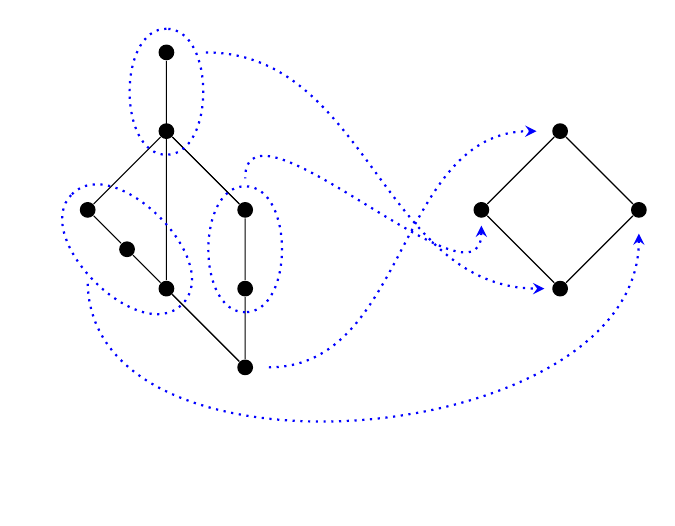
\begin{tikzpicture}[every node/.style={ circle, fill=black, text=black, inner sep=0pt, minimum size=2mm, font=\scriptsize }]
		\node (0) at (0,-2) {};
		\node (1) at (-1,-1) {};
		\node (2) at (-1.5, -0.5) {};
		\node (3) at (-2,0) {};
		\node (4) at (-1,1) {};
		\node (5) at (-1,2) {};
		\node (6) at (0,0) {};
		\node (8) at (0,-1) {};
		\draw (0) -- (1) -- (2) -- (3) -- (4) -- (6);
		\draw (1) -- (0) -- (8) -- (6) -- (4) -- (5) -- (1);

		\node (A) at (4,-1) {};
		\node (B) at (3,0) {};
		\node (C) at (5,0) {};
		\node (D) at (4, 1) {};
		\draw (A) -- (B) -- (D) -- (C) -- (A);
		\draw[blue, dotted, line width=0.8pt] (0,-1.3) to[out=180, in=180] (0,0.3) to[out=0, in=0] (0,-1.3);
		\draw[blue, dotted, line width=0.8pt] (-2.2,0.2) to[out=45, in=45] (-0.8,-1.2) to[out=-135, in=-135] (-2.2,0.2);
		\draw[blue, dotted, line width=0.8pt] (-1,2.3) to[out=180, in=180] (-1,0.7) to[out=0, in=0] (-1,2.3);
		\draw[blue, dotted, -stealth, line width=0.8pt] (0.3,-2) to[out=0, in=180] (3.7,1);
		\draw[blue, dotted, -stealth, line width=0.8pt] (-0.5,2) to[out=0, in=180] (3.8,-1);
		\draw[blue, dotted, stealth-, line width=0.8pt] (3,-0.2) to[out=270, in=90] (0,0.4);
		\draw[blue, dotted, stealth-, line width=0.8pt] (5,-0.3) to[out=270, in=270] (-2,-0.9);
	\end{tikzpicture}

	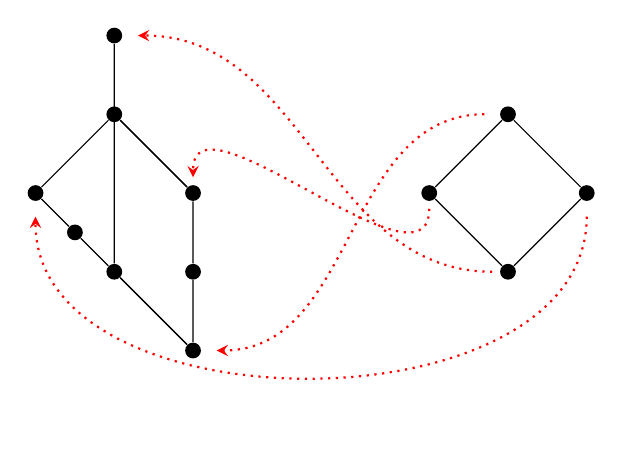
\begin{tikzpicture}[every node/.style={ circle, fill=black, text=black, inner sep=0pt, minimum size=2mm, font=\scriptsize }]
		\node (0) at (0,-2) {};
		\node (1) at (-1,-1) {};
		\node (2) at (-1.5, -0.5) {};
		\node (3) at (-2,0) {};
		\node (4) at (-1,1) {};
		\node (5) at (-1,2) {};
		\node (6) at (0,0) {};
		\node (8) at (0,-1) {};
		\draw (0) -- (1) -- (2) -- (3) -- (4) -- (6);
		\draw (1) -- (0) -- (8) -- (6) -- (4) -- (5) -- (1);
		\node (A) at (4,-1) {};
		\node (B) at (3,0) {};
		\node (C) at (5,0) {};
		\node (D) at (4, 1) {};
		\draw (A) -- (B) -- (D) -- (C) -- (A);
		\draw[red, dotted, -stealth, line width=0.8pt] (3.7,1) to[out=180, in=0] (0.3,-2);
		\draw[red, dotted, -stealth, line width=0.8pt] (3.8,-1) to[out=180, in=0] (-0.7,2);
		\draw[red, dotted, -stealth, line width=0.8pt] (3,-0.2) to[out=270, in=90] (0,0.2);
		\draw[red, dotted, -stealth, line width=0.8pt] (5,-0.3) to[out=270, in=270] (-2,-0.3);
	\end{tikzpicture}
	\caption{A Galois connection} \label{figure:Galois-connection}
\end{figure}

That is, if we consider the map $\varphi$ from the closure system on $\mathbf{X}$, it is infact surjective
(\textit{onto}) the closure system induced for $\mathbf{Y}$. Likewise, $\psi$ is surjective to the closure system
on $\mathbf{X}$. Consider two elements $x,x'$ of the closure system on $\mathbf{X}$ so that $\varphi(x) =
	\varphi(x')$. We may construct the equality $x = \psi \big(\varphi (x)\big) = \psi\big (\varphi(x')\big) = x'$
which shows that each map is additionally injective (\textit{one-to-one}), and so also a bijection. That they are
order-reversing can be seen from , and so we have a dual isomorphism.

\Cref{figure:Galois-connection} demonstrates a rather contrived Galois connection between two partially ordered
sets. Generally, Galois connections are interesting when the closure systems they induce are interesting in their
own right. We will wait until \Cref{chapter:formal-concept-analysis} to see an example of this.

\section{Propositional Logic}
\label{section:propositional-logic}

Propositional logic is a system for abstracting reasoning away from natural language. A \textit{propositional
	statement} is a sentence like \say{Tralfamadorians have one eye}. That is, something that may be assigned a value
of \textit{true} or \textit{false} \cite{Ben1993Mathematical}. More complex propositions may be constructed
recursively from simpler ones. The main interest is then to discover which true propositions follow---under some
agreeable sense of what it means to \textit{follow}---from others.

\subsection{Syntax}
\label{subsection:syntax} \index{propositional logic} \index{propositional logic!syntax} \index{boolean operators}
\index{propositional logic!atom}

\textit{Propositional atoms} are the fundamental building blocks of a propositional language. They are indivisible
statements that can either be true or false, and may be be combined with the boolean connectives $\{\neg, \lor,
	\land, \rightarrow \}$ to construct more complex statements, or \textit{formulae}. Respectively, we refer to
$\neg$ as \textit{negation}, $\vee$ as \textit{disjunction}, $\wedge$ as \textit{conjunction}, and $\rightarrow$
as \textit{material implication}. Propositional atoms are denoted with lower-case Latin letters $p,q,r,s,$ and
$t$, and the set of all atoms will usually be denoted by $\mathcal{P}$. Lower-case Greek letters $\alpha, \beta,
	\gamma, \phi, \psi,$ and $\phi$ will be used to denote formulae, and corresponding upper-case Greek letters will
usually represent sets of formulae.

Not all combinations of atoms and Boolean connectives result in meaningful expressions. For example, ``$\land
	\rightarrow \phi$,'' which can be parsed as \say{Conjunction materially implies $\phi$}, has no discernible
meaning. We distinguish between any formula and so-called \textit{well-formed formulae}. The latter being
constructions that are valid with respect to the rules of the grammar defined inductively in Backus--Naur form
below \cite{Huth_Ryan_2004}.
%
\begin{align*}
	\phi ::= p \mid (\neg \phi) \mid (\phi_{1}\lor \phi_{2}) \mid (\phi_{1}\land \phi_{2}) \mid (\phi_{1}\rightarrow \phi_{2}) \mid (\phi_{1}\leftrightarrow \phi_{2})
\end{align*}

We are entirely uninterested in formulae that are not well-formed, so we drop the suffix ``well-formed'' under the
recognition that we shall never again mention the alternative \cite{Huth_Ryan_2004}.

Any formula accepted by this grammar is said to be in the language $\mathcal{L}^{\mathcal{P}}$, although we may
also drop the superscript where possible. To make reading this dissertation slightly more enjoyable, we may
construct examples where we denote propositional atoms by monospaced text, enabling the expression of formulae
suggesting a more interesting domain, such as $\texttt {tralfamadorians}\rightarrow \neg \texttt{human}$, which
should be interpreted as proposing that \say{Tralfamadorians are not human} \cite{vonnegut1969slaughterhouse}.

\subsection{Semantics}
\label{subsection:semantics} \index{propositional logic!semantics}

In the previous subsection we described the role that the syntax of propositional logic plays, and how the boolean
connectives facilitate the construction of arbitrarily complex formulae from atoms. However, aside from this
description of the form of propositional languages, nothing about their meaning has been discussed; as of yet, we
are not equipped to answer the question of when a formula must be true. This is the role of semantics.
Specifically, the aim is to show how the truth of an arbitrary formula may be defined relative to truth
assignments to propositional atoms. We will then describe how understanding the semantics of propositional logic
allows one to describe the idea of logical consequence: when the truth of certain formulae necessitate the truth
of another.

Propositional atoms were described as indivisible statements that are assigned values of \textit{true} or
\textit{false}. We now define a function that assigns a truth value to each atom in the set $\mathcal{P}$ of
atoms. \index{propositional logic!valuations}

\begin{definition}
	\label{definition:valuation} \index{propositional logic!semantics!valuations}

	A \textit{valuation} is a function $u : \mathcal{P}\to \{\textit{ true}, \textit{ false }\}$ that assigns a truth
	value to each propositional atom.
\end{definition}

Given a set of atoms $\mathcal{P}= \{p,q,r\}$, we write $\mathcal{U}$ to denote the set of all possible
valuations. A valuation $u \in \mathcal{U}$ \textit{satisfies} an atom $p \in \mathcal{P}$ if $u$ maps $p$ to
\textit{true}, and so we write $u \vDash p$. Otherwise, we write $u \nvDash p$ to indicate that $u$ does not
satisfy $p$ (in this context, meaning $u$ maps $p$ to \textit{false}) \cite{Ben1993Mathematical}. It is often
easier to represent valuation functions by describing them as the set of atoms in their domain, with identifiers
for truth values. We may then write $\{\, p,q,\overline{r}\,\}$ to refer to the valuation that maps $p$ and $q$ to
true, but $r$ to false.

This satisfaction relation can be extended beyond propositional atoms to include more complex formulae, as
described in \Cref{subsection:syntax}. For any $\phi, \psi \in \mathcal{L}$,
\begin{itemize}
	\item $u \vDash \neg \phi$ if and only if $u \nvDash \phi$ \hfill (negation)

	\item $u \vDash \phi \vee \psi$ if and only if $u \vDash \phi$ or $u \vDash \psi$ \hfill (disjunction)

	\item $u \vDash \phi \wedge \psi$ if and only if $u \vDash \phi$ and $u \vDash \psi$ \hfill (conjunction)

	\item $u \vDash \phi \rightarrow \psi$ if and only if $u \vDash \neg \phi$ or $u \vDash \psi$ \hfill (material implication)

	\item $u \vDash \phi \leftrightarrow \psi$ if and only if $u \vDash \phi \rightarrow \psi$ and $u \vDash \psi \rightarrow \phi$ \hfill (material equivalence)
\end{itemize}

Following the idea of what it means for a formula to be satisfied, we have,

\begin{definition}
	\label{definition:model} \index{propositional logic!semantics!model}

	For a valuation $u \in \mathcal{U}$ and formula $\phi \in \mathcal{L}$ we call $u$ a \textit{model} of $\phi$ if
	and only if $u$ satisfies $\phi$. The set of all models of $\phi$ is constructed by $\hat{\phi}\coloneqq \{u \in
		\mathcal{U}\mid u \vDash \phi \}$.
\end{definition}

Satisfiability can be extended to sets of formulae in such a way that a valuation $u \in \mathcal{U}$
\textit{satisfies} the set $\Phi \coloneqq \{\phi_{0}, \ldots, \phi_{n}\}$, and so is a model of it, when $u
	\vDash \phi_{i}$ for all $0 \leq i \leq n$, and we write $u \vDash \Phi$. If $\Phi$ has no model then it is
\textit{unsatisfiable} \cite{Ben1993Mathematical}.

\begin{definition}
	\label{definition:compactness} \textbf{INSERT COMPACTNESS}
\end{definition}

\subsection{Logical Consequence}
\label{subsection:logical-consequence} \index{propositional logic!consequence}

The introduction of models at the end of \Cref{section:propositional-logic} leads quite naturally into a
discussion on the matter of \textit{logical consequence}, which provides an answer---in terms of the
semantics---to the question of when it is appropriate to infer one formula from another
\cite{tarski1936consequence}.

For example, if we know that \say{\textit{Billy Pilgrim lived in Slaughterhouse 5}} and that \say{\textit{The
		inhabitants of Slaughterhouse 5 survived the bombing of Dresden}}. We may then hold the view that, as a result of
these two pieces of knowledge, it would be sensible to infer that \say{\textit{Billy Pilgrim survived the bombing
		of Dresden}}. Of course, this inference being \textit{sensible}---under some common concept of consequence---gives
little insight into how logical consequence may be appropriately be formalised. It may help one's intuition to try
imagine a world where the first propositions are true while the final one false.

\index{object language} \index{metalanguage} We place a brief moratorium on this discussion to introduce the
notions of the \textit{object} and \textit{metalanguage}. In the scenario that has just been described, the
italicised sentences form a part of the object language: the language we use to model the world and represent
information. The metalanguage facilitates reasoning about elements in the object language. That is, we can use the
metalanguage to describe one sentence being a consequence of another (where these sentences are elements in the
object language). Here, \textit{consequence} is an element of the metalanguage \cite[p 22]{Ben1993Mathematical}.

In this case, both the object and metalanguage are comprised of English, which can certainly lead to confusion.
The distinction is clearer in propositional logic: constructions derived from combinations of atoms and the
boolean operators result in elements of the object language; while the metalanguage uses symbols like $\vDash$ and
$\vdash$, which are introduced below.

\begin{definition}
	\label{definition:logical-consequence}

	Let $\Gamma$ be a set of formulae and $\varphi$ a formula in the language $\mathcal{L}$. We say that $\varphi$ is
	a \textit{logical consequence} of $\Gamma$, and write $\Gamma \vDash \varphi$, if and only if every model of
	$\Gamma$ is a model of $\varphi$, or equivalently if $\hat{\Gamma}\subseteq \hat{\varphi}$.
\end{definition}

This semantic account of consequence, due to Tarski \shortcite{tarski1936consequence}, makes implicit the view
that if $\varphi$ is indeed a consequence of $\Gamma$, then it should not be possible for all the sentences
(formulae) in $\Gamma$ to be true while $\varphi$ be false.

\begin{example}
	\label{example-logical-consequence}

	Ifthe earlier example were modelled in propositional logic, we might initialise \textit{Billy Pilgrim} with
	\texttt{b}, \textit{slaughterhouse 5} with \texttt{h}, and \textit{survived} with \texttt{s}. It is then our aim
	to determine whether $\{\texttt{b}\rightarrow \texttt{h},\; \texttt{h}\rightarrow \texttt{s}\} \vDash
		\texttt{b}\rightarrow \texttt{s}$. From the satisfaction relation in \Cref{subsection:semantics} it can be derived
	that the models of $\{\texttt{b}\rightarrow \texttt{h},\; \texttt{h}\rightarrow \texttt{s}\}$ are precisely:
	\[
		\bigl\{ \{\overline{\texttt{b}},\,\overline{\texttt{h}},\,\overline{\texttt{s}}\}, \{\overline{\texttt{b}},\,\overline{\texttt{h}},\,{\texttt{s}}\}, \{\overline{\texttt{b}},\,{\texttt{h}}
		,\,{\texttt{s}}\}, \{{\texttt{b}},\,{\texttt{h}}, \,{\texttt{s}}\} \bigr\}.
	\]
	These are indeed all models of $\texttt{b}\rightarrow \texttt{s}$, and so we answer the question in the affirmative.
\end{example}

\textit{Consequence operators} are functions over a given language that map sets of formulae to the set of all
their consequences. They were introduced by Tarski \shortcite{tarski1936operator} as the symbol $\cons$
representing a general idea that sets can be closed under a specified notion consequence. In future, we use
$\cons$ to refer specifically to closure under classical (\textit{Tarskian}) consequence; and so, application of
the $\cons$ operator to a set $\Gamma$ would yield $\cons (\Gamma ) \coloneqq \{\varphi \mid \Gamma \vDash
	\varphi\}$. Where we wish to reference closure under a different notion of consequence, suppose that of a Hilbert
system, we will use a subscript to denote the system $\cons_{\mathcal{H}}$. To refer to the general notion of
closure under \textit{some} notion of consequence, we write $\cons_{X}$ \cite{citkin2022consequence}.

A \textit{theory} is a set of formulae $\Gamma$ that equals its closure $\cons_{X}(\Gamma)$, it is then said that
$X$ is \textit{deductively closed}. The study of such operators is useful in its ability to reveal properties
about the respective notion of consequence. Indeed, a consequence operator is a closure operator and satisfies
\begin{align}
	\text{(Inclusion)}    & \quad \Gamma \subseteq \cons (\Gamma)                                                \\
	\text{(Idempotency)}  & \quad \cons (\Gamma) = \cons (\cons (\Gamma))                                        \\
	\text{(Monotonicity)} & \quad \Gamma \subseteq \Gamma' \Rightarrow \cons (\Gamma) \subseteq \cons (\Gamma').
\end{align}

\textit{Inclusion} is a relatively easy property to justify with respect to logic consequence. All that it
enforces is that to close a set of formulae under logical consequence---that is, include every statement that
logically follows---one should retain at least the statements that were started with. \textit{Idempotency}
requires that the supposed set of all consequences is indeed the set of \textit{all} consequences.

\subsection{Deductive Systems}
\label{subsection:deduction-systems} \index{Deductive system} \index{Rule of inference}

Logical consequence, described in \Cref{subsection:logical-consequence}, offers a purely semantic account of how
it might be inferred that one formula follows (logically) from another set thereof. In contrast, deductive systems
answer this question syntactically by describing a system of \textit{axiomata} and \textit{rules of inference}
that affirm the truth of one formula from the truth of others \cite[p. 49]{Ben1993Mathematical}.

\begin{definition}
	\label{definition:deductive-system}

	A \textit{deductive system} is a collection of axiomata and rules of inference. A \textit{proof} in such a system
	is a sequence of formulae where each formula is either an axiom, or has been inferred by application of an
	inference rule to previous formulae in the sequence. The final formula in the sequence, $\phi$, is called the
	\textit{theorem} and is then \textit{provable}, and so we write $\vdash \phi$.

	A \textit{theory} (or, \textit{deductively closed theory}) in a deduction system is a set of formulae closed under
	application of axioms and inference rules of the system; and so a set of formulae $\Gamma$ is a theory if it is
	equal to its deductive closure $\cons_{\mathcal{H}}(\Gamma) \coloneqq \{\varphi \mid \Gamma \vdash \varphi \}$. As
	before, elements of a theory are called theorems.
\end{definition}

Deductive systems offer some advantages over their semantic counterparts; particularly, when reasoning over
large---possibly infinite---domains, logical consequence can become difficult. Moreover, semantic consequence
provides little insight into the relationships between pieces of information that lead to the inferences we make;
while the sequential nature of deduction systems trace a path describing this relationship
\cite{Ben1993Mathematical}.

\subsubsection{Hilbert Systems}
\label{subsubsection:hilbert-systems} \index{Deductive system! Hilbert system}

A propositional Hilbert system $\mathcal{H}$ is characterised by three axiom schemata,
\begin{align}
	\text{(Axiom 1)}\quad & \vdash (\phi \rightarrow (\psi \rightarrow \phi)),                                                                               \\
	\text{(Axiom 2)}\quad & \vdash (\phi \rightarrow (\psi \rightarrow \gamma)) \rightarrow ((\phi \rightarrow \psi) \rightarrow (\phi \rightarrow \gamma)), \\
	\text{(Axiom 3)}\quad & \vdash (\neg \phi \rightarrow \neg \psi) \rightarrow (\phi \rightarrow \psi),
\end{align}
and a single rule of inference:
\begin{align}
	\index{Rule of inference! \textit{modus ponens}}\text{(Modus Ponens)}\quad & \frac{\vdash \phi, \qquad \vdash \phi \rightarrow \psi}{\vdash \psi}.
\end{align}
The axiom schemata themselves are not axioms, but rather patterns containing meta-variables that, when uniformly
substituted for formulae, result in an instantiated axiom. The turnstile symbol ($\vdash$) is the syntactic
counterpart to the double-turnstile ($\vDash$) used for logical consequence. We frequently express that $\phi$ is
a theorem by writing $\vdash \phi$ \cite[p. 55]{Ben1993Mathematical}.

As it stands, constructing proofs from instances of axiom schema and applications of modus ponens is a challenging
ordeal. As an illustration, we provide the following Hilbert-style proof for the inference made in
\Cref{example-logical-consequence}.

\begin{example}
	We demonstrate a Hilbert-style derivation of $\texttt{b}\to \texttt{s}$ from the assumptions $\texttt{b}\to \texttt{h}$ and $\texttt{h}\to \texttt{s}$.

	\begin{proofH}
		\label{proof:transitivity}

		\Hstep[Premise]{\vdash (\texttt{b} \rightarrow \texttt{h})} \Hstep[Premise]{\vdash (\texttt{h} \rightarrow \texttt{s})} \Hstep[Axiom 1]{\vdash (\texttt{h} \rightarrow \texttt{s}) \rightarrow (\texttt{b} \rightarrow (\texttt{h} \rightarrow \texttt{s}))}
		\Hstep[MP 2,3]{\vdash (\texttt{b} \rightarrow (\texttt{h} \rightarrow \texttt{s}))} \Hstep[Axiom 2]{\vdash (\texttt{b} \rightarrow (\texttt{h} \rightarrow \texttt{s})) \rightarrow ((\texttt{b} \rightarrow \texttt{h}) \rightarrow (\texttt{b} \rightarrow \texttt{s}))}
		\Hstep[MP 4,5]{\vdash (\texttt{b} \rightarrow \texttt{h}) \rightarrow (\texttt{b} \rightarrow \texttt{s})} \Hstep[MP 1,6]{\vdash (\texttt{b} \rightarrow \texttt{s})}
	\end{proofH}
\end{example}
\textit{Derived rules} are introduced as a means to make it easier to spot the next step in a proof sequence. Of
particular importance is the so called \textit{deduction theorem}, which facilitates the construction of proofs
that are conditioned on a hypothesis, without requiring that the hypothesis be an axiom. \index{Rule of inference!
	deduction theorem}
\begin{align}
	\label{axiom:deduction-theorem}\text{(Deduction Theorem)}\quad & \frac{\Delta \cup \phi \vdash \psi}{\Delta \vdash \phi \rightarrow \psi}
\end{align}
As an illustration, the proof in \Cref{proof:transitivity} can be restated using the \textit{transitivity} derived
rule:
\begin{align}
	\text{(Transitivity)}\quad & \frac{\Delta \vdash \varphi \rightarrow \psi, \qquad \Delta \vdash \psi \rightarrow \gamma}{\Delta \vdash \varphi \rightarrow \gamma}
\end{align}

Derived rules must be sound with respect to what can be proved by the three axioms and applications of modus
ponens. That is, a derived rule should not enable one to make an inference that would not be possible without such
a rule.

The fact that it was able to be shown that \say{Billy Pilgrim survived the bombing of Dresden} through both
semantic and syntactic notions of consequence is not a coincidence. This correspondence between logical
consequence and Hilbert-style deduction systems holds in general for propositional logic (and, in fact for many
other systems with relatively limited expressive power). We capture this correspondence more formally through the
notions of \textit{soundness} and \textit{completeness}.

\begin{definition}
	\label{definition:completeness-hilbert} \index{propositional logic!completeness}

	Given a set of formulae $\Gamma$ and one $\gamma$ in $\mathcal{L}$, $\Gamma \vdash \gamma$ if and only if $\Gamma
		\vDash \gamma$. Where $\vDash$ and $\vdash$ are used in the context with which they have been introduced.
\end{definition}

The proofs for \Cref{definition:completeness-hilbert} are well-known, and can be found in
\cite{Ben1993Mathematical}.

\label{subsubsection:gentzen-systems} \index{Genzten systems}

\subsection{Consequence Relations}
\label{subsection:consequence-relations} \index{consequence relations}

In the preceding sections, the notion of consequence put forward by discussion(s) about the semantics or deductive
system of a particular logic might instead be considered from the more abstract perspective of \textit{consequence
	relations}. In this sense, one considers a relation between formulae in the object-language. The task is then,
just as was done in the definition of partial orders, to study which properties these consequence relations
satisfy. It is these properties which provide a more general characterisation of how consequence behaves in the
respective logic. That is, we may use them to illuminate the pattern and style of reasoning the logic enforces.

When discussing consequence relations we will reuse notation and denote the relation with ``$\vdash$'' (relying on
the surrounding context to disambiguate consequence relations from proof derivations). At times of potential
confusion, a particular consequence relation may be distinguished with a subscript that references the respective
system.

\begin{definition}
	\label{definition:consequence-relations}

	A \textit{consequence relation} $\vdash \; \subseteq \mathcal{L}\times \mathcal{L}$ is a binary relation over a
	formal language that satisfies the following properties:
	\begin{align}
		\text{(Reflexivity)}\quad  & \varphi \in \Gamma \timpls \Gamma \vdash \varphi                                                    \\
		\text{(Monotonicity)}\quad & \Gamma \vdash \varphi \tand \Gamma \subseteq \Psi \timpl \Psi \vdash \varphi                        \\
		\text{(Cut)}\quad          & \Gamma \vdash \Delta, \Psi \tand \Psi, \Phi \vdash \Omega \timpl \Gamma, \Phi \vdash \Delta, \Omega
	\end{align}
\end{definition}

We can view a consequence relation as a set of ordered pairs $\{(\Gamma_{0}, \varphi_{0}), \ldots, (\Gamma_{n},
	\varphi_{n}), \ldots\}$. An alternative representation for the inclusion of a pair in the consequence relation,
$(\Gamma, \varphi) \in \; \vdash$ is to use infix notation, and instead write $\Gamma \vdash \varphi$. The
intended meaning of such inclusions is that from $\Gamma$ one may conclude $\varphi$ \cite{citkin2022consequence}.
As such, it may be helpful to refer to $\Gamma$ as the \textit{premise} and to $\varphi$ as the
\textit{conclusion}. The absence of such a pair from the relation, or $\Gamma \not \vdash \gamma$, is understood
to mean that $\gamma$ is not a consequence of $\Gamma$.

This is a much more significant abstraction on the matter of consequence, requiring no concrete proof system or
semantics. The point is not at all to replace either of these, but rather that one's intuition for how a
particular logic's notion of consequence behaves is frequently much simpler when viewed as properties of a
relation. Later on, in \Cref{chapter:defeasible-reasoning}, we explore the construction of a logic that uses
consequence relations as a starting point to build a semantics around.
